
\documentclass[12pt]{article} %other options include letter and book
% One can also make presentation slides using the 'beamer' class
\usepackage[english]{babel}

% Set page size and margins
% Replace `letterpaper' with `a4paper' for UK/EU standard size
\usepackage[letterpaper,top=2cm,bottom=2cm,left=3cm,right=3cm,marginparwidth=1.75cm]{geometry}

% Useful packages
\usepackage{amsmath,amssymb,latexsym} % gives some additional math symbols and environments
\usepackage{graphicx} % for including graphics
\usepackage[colorlinks=true, allcolors=blue]{hyperref}

% After all the settings and usepackage commands, begin the document

\begin{document}

Here are some problems for Monday, 9 May, 2023.
\bigskip

\begin{enumerate}
\setlength{\itemsep}{20mm} % increases spacing between list items

\item (This is problem 4.30 from the textbook.) A graph is called a
  \emph{tree} if can be drawn so that it branches upwards and none of
  its branches intersect. Two examples of a tree are shown in
  Fig.~\ref{fig:tree}. Prove that if a tree has $n$ vertices, then it
  has $n-1$ edges.

\begin{figure}[h]
  \centering
\vspace{2mm}
  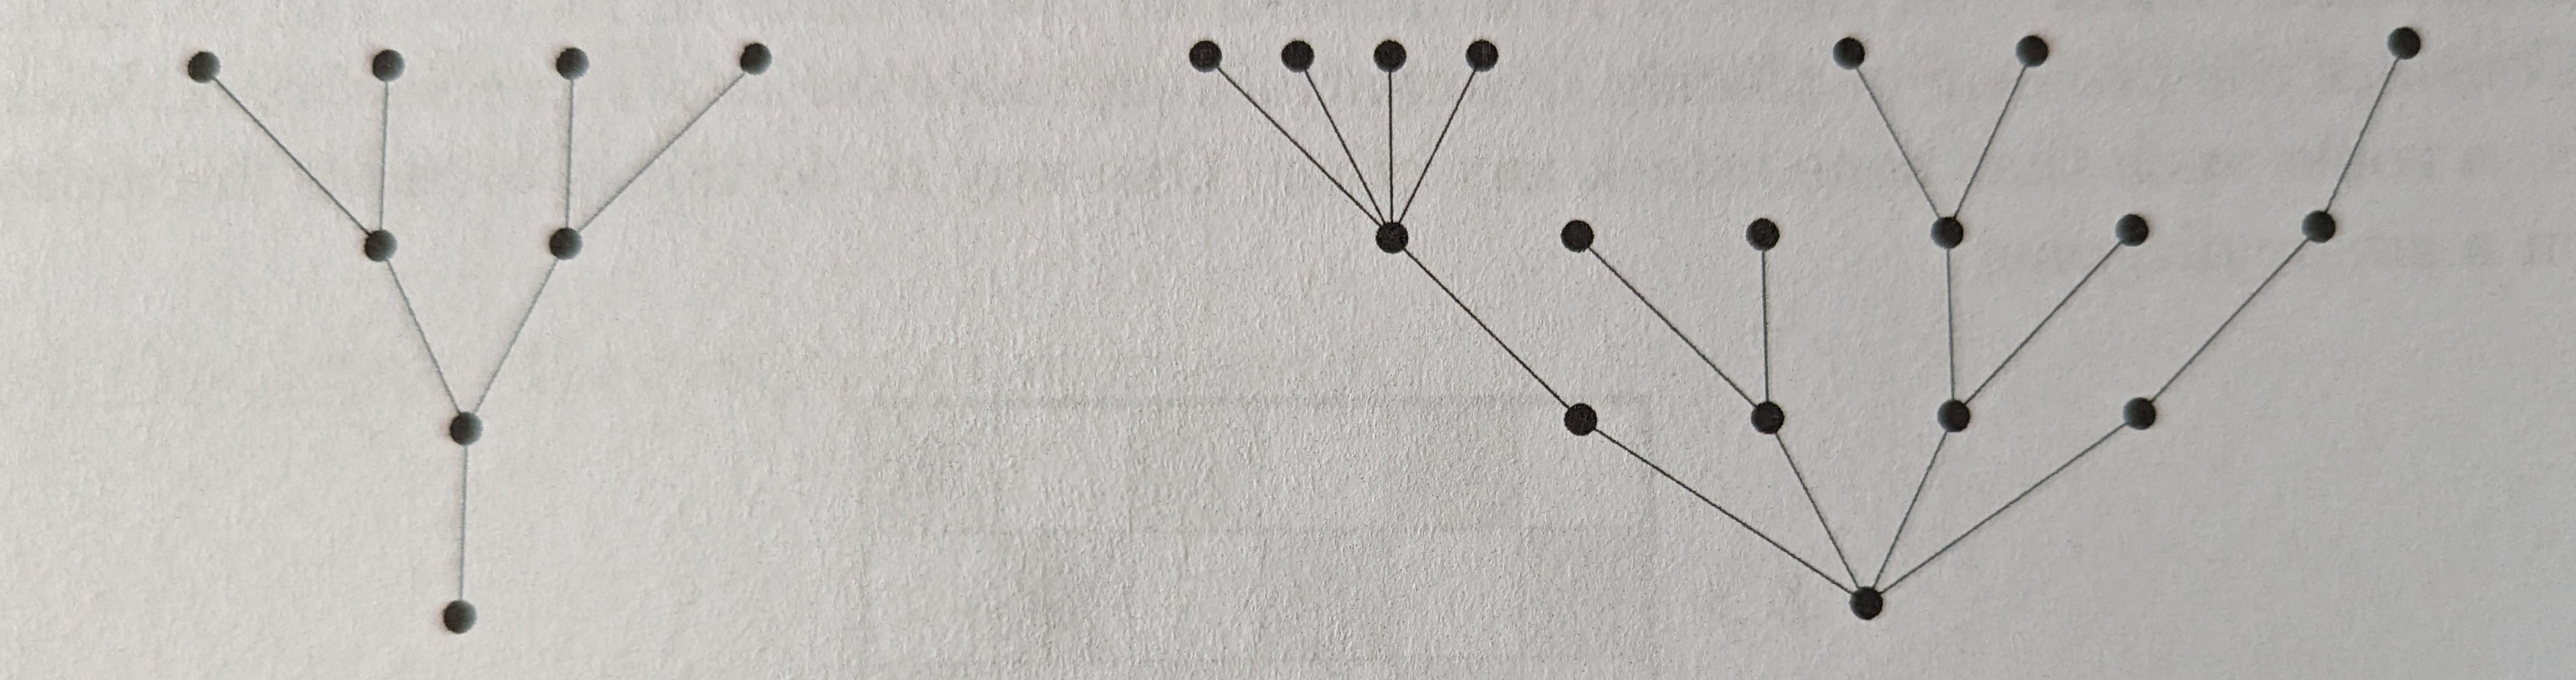
\includegraphics[width=4in]{tree.jpg}
\caption{Figure from \emph{Proofs} by Jay Cummings, page 150.}
\label{fig:tree}
\end{figure}



\item Prove that $3^{5n} - 5^{3n}$ is divisible by $59$ for any $n \in
  \mathbb{N}$. 


  
\item {\bf Optional!} Possibly challenging. Possibly interesting. I
  dunno.  Given a positive integer $s_1$, let $s_2$ be the sum of the
  squares of the digits of $s_1$. Let $s_3$ be the sum of the squares
  of $s_2$, and so on. Prove that for any choice of $s_1$, the
  sequence $(s_1, s_2, s_3, \ldots )$ eventually reaches either $1$ or
  $42$. 

  
\end{enumerate}




\end{document}
